% ----------------------------------------------------------------
% Article Class (This is a LaTeX2e document)  ********************
% ----------------------------------------------------------------
\documentclass[12pt]{article}
\usepackage[english]{babel}
\usepackage{amsmath,amsthm}
\usepackage{amsfonts}
\usepackage{xltxtra,xcolor,url}
\usepackage{ctex}
\usepackage{mathptmx}   %是英文字体为Times New Roman
\usepackage{tabu}  %表格
\usepackage{booktabs}   %表格
\usepackage{multirow}   %表格合并
\usepackage{multicol}   %表格合并
\usepackage{longtable}  %表格合并
\usepackage{rotating}   %表格合并
\usepackage[top=30mm, bottom=20mm, left=30mm, right=30mm]{geometry}  %页面边距设置
\usepackage{graphicx}   %插图
% THEOREMS -------------------------------------------------------
\newtheorem{thm}{Theorem}[section]
\newtheorem{cor}[thm]{Corollary}
\newtheorem{lem}[thm]{Lemma}
\newtheorem{prop}[thm]{Proposition}
\theoremstyle{definition}
\newtheorem{defn}[thm]{Definition}
\theoremstyle{remark}
\newtheorem{rem}[thm]{Remark}
\numberwithin{equation}{section}
% ----------------------------------------------------------------
\begin{document}

\title{新人扫盲帖}
\author{(欢迎大家指正并修改)}
\date{2014年}
% ----------------------------------------------------------------

\maketitle
\huge\textcolor{red}{严禁一切作弊---飞机(fakeGps)、互刷等行为。一旦发现,全体举报!}
% ----------------------------------------------------------------
\normalsize
\newpage
首先欢迎大家加入绿军大家庭!ingress是一个需要点探索精神和脱宅毅力的游戏~所以多出门是必要、必须、必做到的大大大前提。如果你懒得出门,懒得研究~个人建议,不如在家里玩玩PS3或者魔兽神马的,有空调、可乐、炸薯条的日子也是很美好滴!下面写的,也基本都是些技巧、窍门之类的。 看不懂的词,请查阅中文网(尤其英文不好的童鞋们),百度贴吧里则有很多新手提问,应该能解决大部分游戏进不去神马的这类问题。建议新手多多利用搜索功能,不要坐定伸手党 :)

\section{关于流量}
这是个问题~~要说一个月包多少呢,我也不好说,看你玩的程度。这里教大家一个省流量的方法,就是google map有一个离线下载的功能,允许在离线状态下使用。还是可以省下不少的哟!:) 我上下班路上扫扫po,给po充充电啥的,大概20M每天。稍微多走点地方,就30-40M(2014年)。这个大家根据自己情况可以估算一下。另外一般各高校开学,移动和联通都会有很多划算的套餐办理,具体移动和联通的优惠信息大家可以在群里咨询,会有很多小伙伴提供信息给你。
-------------
在2018年流量应该不是个问题了吧。
\section{关于XM}
就是你地图上看的小白点~游戏界面上,横在最上面的那一条长得像血槽的东东~它是游戏里你一切动作的能量条!根据等级增长会有定额增长。获取方法就是溜达~还有可贵的power cube以及回收道具。

\section{关于Hack}
敌我双方的portal在距离范围内,都可以hack!敌方给100ap~相对来说道具少一些。友方不给ap,但道具会多一些。道具等级,是取你和塔比较低那一方限制~比如你3级,hack 8级塔也不会得到8级道具!可能RP爆发会得到5级。长按hack会进入画图小游戏界面,界面会先出现一些图形然后让你再按顺序一一画出,如果画对会有额外的道具奖励,一般对的越多画的越快得到的道具就越多(群文件里有画图小插件可以帮助你练习)。Hack时会出现一个叫portal key的东西,这是完成link的必备物品,但是如果你已经有这个portal的key,那么再次hack就不会出了。所以如果你希望得到多把同一个portal的key,可以(1)将已经得到的这个portal的key扔到地上,这个要特别注意你周围是否有敌军,不要被别人捡走啦;(2)将这个portal的key放进胶囊capsule里面,然后再hack。注意:得到portal key也是要很人品的哦!

\section{关于Deploy}
1级res每人每塔可以放8只。2~4级的放4只。5~6级放2只。7~8级放1只。Res 的远近,是你离portal中心的位置,最理想距离是portal压着你的范围绿圈~这样摆出来res最远,至于为啥要这样摆呢?我们都知道XMP的攻击是随着距离增加而递减的,so~摆放越开,敌军来打就会越费道具。(当然,高级道具攻击范围很远~可习惯是要慢慢养成滴~)\par
修正:由于Ultra Strike的出现,现阶段最优摆放方式为六个res压圈摆放,两个res在18米范围内摆放(us的最小攻击范围)。除掉极其重要的portal为节省时间可全部压圈摆放。

\section{关于Link}
能进行link必须具备以下条件:
\begin{itemize}
\item 需要link的两个portal必须八个角全满;
\item 必须够到link出发点的portal;
\item 必须有被link的portal的key;
\item link出发点的portal的可link距离必须大于两个portal之间的距离;
\item 有link操作需要的XM;
\item 没有其他link的阻挡;
\item 一个Portal可以链出8条Link,链入无上限。
\end{itemize}
注意,portal key是消耗品,创建完一条link就会用掉一个key。
另外,link的距离是由出发portal的等级限制的,请新人额外注意这一点,不要不舍得放你手里的高级腿,portal等级高,随后出的物品也越好哟。 \par
\begin{table}
\begin{center}
\caption{Portal等级与link距离}
\begin{tabular}{ll}
等级 & 最远距离 \\
1 & 160 m \\
2 & 2.56公里  \\
3 & 12.96公里 \\
4 & 40.96公里 \\
5 & 100公里   \\
6 & 207.36公里\\
7 & 384.16公里\\
8 & 655.36公里
\end{tabular}
\end{center}
\end{table}

\section{关于多重Field}
多重field方案的实施是为了利用少量的po创造出更大的field数目,获得更多的ap,是各位agent升级的最佳方案。\par
根据field里的po不能向外link的原则,做多重field需要注意link的方向和顺序。\par
简单的说,四个点最多可以连四个field,这样就形成了一个多重field。如果不注意顺序的话只能连接三个field。下面详细讲一下link的方法。\par
\subsection{多重方法一}
先建一个field(Figure\ref{m11}) \par
\begin{figure}
  \centering
  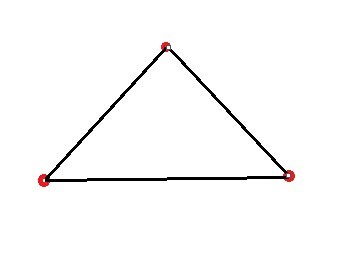
\includegraphics[scale=0.5]{pictures/m11.png}\\
  \caption{先建一个field}
  \label{m11}
\end{figure}
在外围连一个大field盖住原来小的(Figure\ref{m12}) \par
\begin{figure}
  \centering
  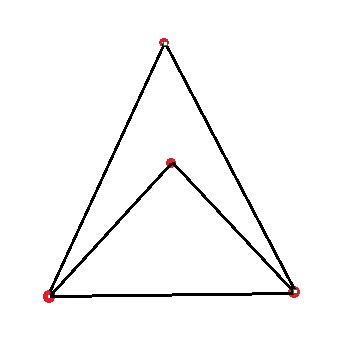
\includegraphics[scale=0.5]{pictures/m12.png}\\
  \caption{在外围连一个大field盖住原来小的}
  \label{m12}
\end{figure}
站在A点link到B点(Figure\ref{m13})
\begin{figure}
  \centering
  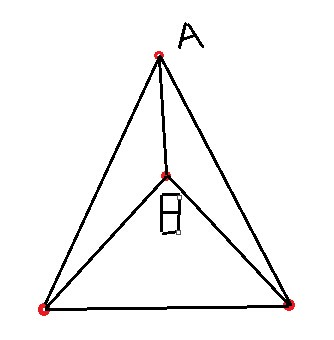
\includegraphics[scale=0.5]{pictures/m13.png}\\
  \caption{站在A点link到B点}
  \label{m13}
\end{figure}
\subsection{多重方法二}
先连一个field,但是里面有一个点(Figure\ref{m21})\par
\begin{figure}
  \centering
  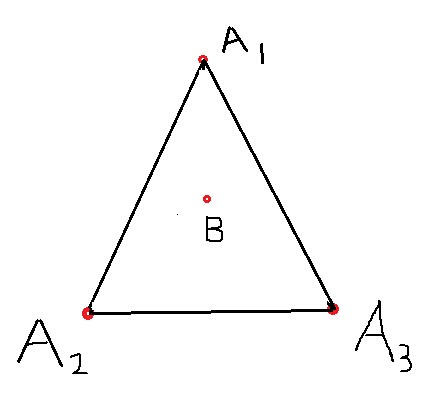
\includegraphics[scale=0.5]{pictures/m21.png}\\
  \caption{先连一个field,但是里面有一个点}
  \label{m21}
\end{figure}
依次站在A1、A2、A3连到B点(Figure\ref{m22})
\begin{figure}
  \centering
  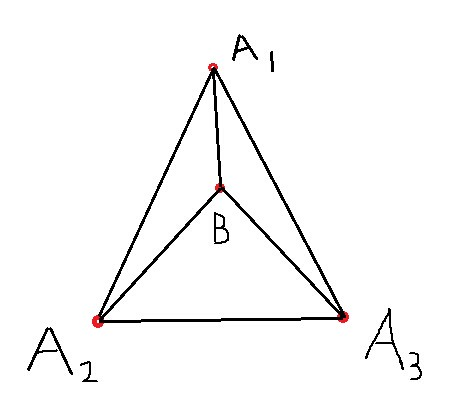
\includegraphics[scale=0.5]{pictures/m22.png}\\
  \caption{依次站在A1、A2、A3连到B点}
  \label{m22}
\end{figure}

\section{关于Recharge}
当本方他能量不满时就可以进行recharge操作,但条件是:(1)你能够的到那个portal 或者有那个portal的key;(2)你的XM够充一次,或者够充一个脚的能量。每次充能有10点AP可拿。\par
Portal能量不足的原因:(1) 自然衰减,这是游戏设定的没法改变,衰减速度一般为每天15\%,但是有活动时衰减速度会有所变化;(2)被敌方攻击。\par
在个人成就里有个recharge和guardian奖章都必须通过此操作才能拿到。

\section{关于Fire}
当要摧毁地方的脚时需要使用XMP进行fire,长按屏幕再点击fire XMP可以快速使用摧毁工具。XMP的等级从1到8威力依次增强,按XMP时自己周围会出现能量环从中间向四周发散,越靠近中间额外增加的威力越强。

\section{关于Drop}
Drop操作可以将物品仓库中的物品丢到地上,丢的地点就是当前的位置(三角的位置)。

\section{关于Recycle}
由于所有物品都是XM的转化形式(请参考剧情),所以所有的物品也可以转化成XM。钥匙回收后的XM值要远大于其他道具,所以一堆钥匙可以当糖吃哦。但是游戏内购后用金钱买的的道具不可以recycle.

\section{关于Passcode}
是通过解析media所得的相当于道具礼包的东东。【G+好像有人给过破解的一些方法,不过我木有研究过,此处不做过多解释,有兴趣的可以去G+翻翻前辈们的帖子】Media有等级之分,越高等级的passcode存活时间越短(因为世界通用)。所以手慢无哦~获得渠道一般去G+有分享群,还有群里随时有人转发!

\section{关于升级}
几乎每一个操作都可以拿到AP,8级之前拥有足够的AP就可以升级,8级之后需要同时满足AP和牌子的要求才能升级。每个玩家agent页面AP数据下就是升级所需要的条件。
XMP炸塔占portal是最基本的。但对于新人我们不建议挑战高级塔,道具和XM都会吃不消,更容易造成废了半天劲打不掉一个res就拿不到一丁点ap!(对,一定要至少打掉一个脚才有ap!)那么hack敌军塔是个很好的升级方法,每个塔每4个小时可以hack4次,就是400ap~帝都现在蓝军人数和活动范围都很大,遍地是蓝portal,所以次方法拿经验同时还能收集不少道具是非常划算的。【你hack它两天就等于它饿了两天。你赚足AP和道具,再回头打它个残血portal~这笔账,你们都懂的算啦:) 】如果你周围绿色portal多,也不用担心,多hack 出key连field!经验大大滴。Key是消耗品,用一个少一个,因此我们建议,在连不成field 的情况下,大家尽量留着key~一次多赚ap(也就是经验)。

\section{关于Mod}
每个portal都有四个mod可以加,一个玩家最多加两个mod。Mod是用来增加portal状态的。现在一一讲解每种mod的用途,其中一些有common,rare, very rare之分,从common,rare到very rare表示其作用越明显。Portal shield用来增加portal的防御能力,敌方攻击时就会减少一定的伤害。Link amp增加portal能link的距离。Heat sink减少hack portal的冷却时间。Multi-hack增加portal在过热之前的hack次数。Force amp增加portal攻击敌方玩家的伤害程度。Turret增加portal攻击敌方玩家的频率。一般作防御的portal mod状态时两个shield+force amp+turret,hack比较多就多加multi-hack。

\section{关于使用Cupsule}
Cupsule可以用来存储物品,每个存储量为100。当需要与其他agent批量交换装备时,先将物品装到cupsule里,然后drop掉让他(她)捡起来。cupsule分rare和very rare 两种,very rare的红色cupsule可以每天按一定的概率复制里面的物品,但是当其满100后就不会复制了。

\section{关于使用Ultra Strike}
Ultra strike 是用来专门摧毁敌方mod(sheild和turrent)的工具,使用方法和XMP相似,可以续能释放,但是攻击范围十分有限,所以使用Ultra strike摧毁mod时要站在po上,即自己的位置和po位置重合,然后释放,效果更佳。

\section{关于申请 Portal}
长按游戏屏幕,会出现NEW PORTAL选项,然后会启动相机拍照,然后点击地图进行位置修正,填写portal名字就完成申请。\par
也可以在游戏外拍照,且照片带有GPS位置信息,然后分享到ingress,点击地图进行位置修正,填写portal名字完成申请。\par
成功提交后会受到确认邮件,进入漫长的审核等待期。现在审核期大概需要四个月(2014.09.05)。\par
但是并不是随意的照片都可以进行申请,具体的申请标准参考官方申请原则。\par
官方的portal申请原则
\url{https://support.google.com/ingress/answer/3066197?hl=zh-Hans&ref_topic=2799270} \par
\large{截至2015年12月22日,申请Portal功能处于关闭状态。}

\section{关于偏移}
国家出于安全考虑,为了不让重要的位置的地理信息暴露,在所有的电子地图服务提供商都需要给地图数据加上偏移和加密,所以我们在使用google,baidu等电子地图服务商的地图时,就会发现显示在地图上的位置和实际的位置不一致的情况。卫星图没有偏移量问题,卫星图不在地图的范畴中。\par
但是在游戏里人物和P点是一起偏的,所以只是街道不对,但P点和你的相对位置是正确的,所以只要在现实里走到位置,在游戏里也就到位了。也就是说,在http://ingress.com/intel中查看卫星地图、记录位置,然后在现实中走过去就好了。\par
2017年底的一次更新解决了中国大陆位置偏移的问题,中国玩家终于可以开始使用游戏里的地图了。
\section{关于搭梯}
想要玩ingress进行翻墙是必须具备的条件,翻墙的方法也有很多,下面从Android和IOS两个方面分别详细说明。

\subsection{Android}
\subsubsection{fqrouter2}
fqrouter2是一个非常好用的且比较稳定的免费App,手机无需root(当然root了功能更全)。Google play商店地址:\\
\url{https://play.google.com/store/apps/details?id=fq.router2} \par
另赠送一个google play商店apk安装包下载地址,只需要将google play商店中的app网址输入即可下载apk安装包:\\
\url{http://apps.evozi.com/apk-downloader/}
\subsubsection{修改hosts文件}
用这种方法的前提是手机已root!\par
将下载到的hosts文件粘贴到/system/etc/hosts,可以使用root explorer等文件管理App进行操作。\par
Root explorer下载地址:\\
\url{https://play.google.com/store/apps/details?id=com.clearvisions.explorer}\par
完成后就可以愉快地游戏了。\par
但是hosts不稳定,需要经常更换。如果不想手动更换,安装SmartHosts这个App可以自动更新hosts。\par
SmartHosts下载地址:\\
\url{https://play.google.com/store/apps/details?id=mobi.smarthosts}

\subsubsection{Shadowsocks}
Shadorsocks Google Play商店地址:\\
\url{https://play.google.com/store/apps/details?id=com.github.shadowsocks}\par
可以购买Shadorsocks服务或者,使用Shadorsocks公益账号:\\
\url{https://www.shadowsocks.net/}

\subsubsection{VPN}
首先得有一个VPN账号,有很多免费的和付费的。\textcolor{red}{(需要临时VPN账号的可以到群里找Agent hackCN,大神主动帮助哦。)}\par
然后在手机上设置VPN就可以了。还是不会的话请点传送门\\
\url{https://www.google.com/webhp?sourceid=chrome-instant&ion=1&espv=2&es_th=1&ie=UTF-8#newwindow=1&q=android\%20vpn\%E8\%AE\%BE\%E7\%BD\%AE}

\subsection{IOS}
\subsubsection{VPN}
同Android.

\subsubsection{修改hosts文件}
用这种方法的前提是手机已越狱!并安装tsProtecter软件。\par
将下载到的hosts文件粘贴到/etc,可以使用iFile等文件管理App进行操作。\par
完成后就可以愉快地游戏了。但是hosts不稳定,需要经常更换。

\section{常用网站}
\begin{longtable}{ll}
1& \url{http://www.ingress.com/}官网\\
2& \url{http://ingresscn.com/}中文网(玩家自译的福利站)\\
3& \url{http://www.ingress.com/intel}地图\\
4& \url{http://iitc.jonatkins.com/}IITC插件(地图插件,注意:非官方插件请慎用)\\
5& \url{http://in-nanjing.com/}一些玩家做的小站,可以提供一些新手Q\&A\\
6& \url{http://tieba.baidu.com/f?kw=ingress}百度ingress吧
\end{longtable}

\section{后记}
本教程主要由Agent Kisukecats编写,Agent JeffHugh辅助编写。多谢Ingress帝都绿军吹水群各位Agents的大力支持和帮助。如文中有错误或不当之处,抑或您有些许想法内容可以分享,欢迎对文档进行修正、增补。\par

文档Github地址:\url{https://github.com/huiselilun/IngressTutorial}\par

帝都绿军QQ群号:214873055 \par
申请加入时请报您的游戏ID(为了防止广告植入)\par

群里不乏各种计算机高手,他们修行甚高,是我等所可望而不可及的。文中最后关于翻墙之术只是皮毛,如想深入了解,请关注各位大神博客。
\begin{longtable}{ll}
 Agent SuperWang & \url{http://superwang.me/}\\
Agent KasuganoHaruka  &\url{http://mrx.im/}\\
 Agent hankCN & \url{http://aa-v.com/}\\
Agent einverne & \url{http://www.einverne.tk/}\\
Agent draplater & \url{http://drapl.me/}
\end{longtable}


\end{document}
% ----------------------------------------------------------------
